%%%%%%%%%%%%%%%%%%%%%%%%%%%%%%%%%%%%%%%%%
%
% In 4073 Embedded Real-Time Systems Course report
% Team 2: Daniel Lemus Perez, Diogo Monteiro and Imara C.T.M. Speek
%
%%%%%%%%%%%%%%%%%%%%%%%%%%%%%%%%%%%%%%%%%

%----------------------------------------------------------------------------------------
%	PACKAGES AND DOCUMENT CONFIGURATIONS
%----------------------------------------------------------------------------------------

\documentclass{article}

\usepackage{graphicx} % Required for the inclusion of images
\usepackage{natbib} % Required to change bibliography style to APA
\usepackage{amsmath} % Required for some math elements 
\usepackage{anysize}
\marginsize{2cm}{2cm}{2cm}{2cm} % decrease the margins

\usepackage{xcolor}
\newcommand\worries[1]{\textcolor{red}{#1}} %add command to specify worries in red
\newcommand\todo[1]{\textcolor{blue}{#1}} % add command to specify todo in blue

\usepackage[toc, page]{appendix} % to include appendices
\usepackage{listings} % to include source code

%\setlength\parindent{0pt} % Removes all indentation from paragraphs

\renewcommand{\labelenumi}{\alph{enumi}.} % Make numbering in the enumerate environment by letter rather than number (e.g. section 6)

%\usepackage{times} % Uncomment to use the Times New Roman font

%----------------------------------------------------------------------------------------
%	DOCUMENT INFORMATION
%----------------------------------------------------------------------------------------

\title{IN4073 Embedded Real-Time Systems \\ QR Lab report - Team II} % Title

\author{Diogo \textsc{Monteiro}, Daniel S. \textsc{Lemus} and Imara C.T.M. \textsc{Speek} \\
		4323688 870754 1506374} % Authors' names

\date{\today} % Date for the report

\begin{document}

\maketitle % Insert the title, author and date

% abstract of 10 lines maximum specifying the specific approach and results
 \begin{abstract}


 \end{abstract}

%----------------------------------------------------------------------------------------
%	INTRODUCTION
%	include the problem statement
%----------------------------------------------------------------------------------------

\section{Introduction}
\label{sec:introduction}


%----------------------------------------------------------------------------------------
%	ARCHITECTURE
%	Specify all software components + interfaces
%----------------------------------------------------------------------------------------

\section{Architecture}
\label{sec:architecture}

This section introduces the QR hardware, their interfaces and the implementation in software components. 


%----------------------------------------------------------------------------------------
%	IMPLEMENTATION
%	How you did it and who did what
%----------------------------------------------------------------------------------------

\section{Implementation}
\label{sec:implementation}

This section introduces the implementation of the functionalities implemented in the system. These concern, GUI communication protocols, safety measures, speed enhancements and basic functionalities.


%-------------------------------------------------------------------------------------------------------------------------------------------------------------------------------------
%GUI
\subsection{GUI}
A simple GUI is designed to control the QR (Figure \ref{fig.GUI}) using QT creator allowing for multi-platform deployment. Users can interact with the QR through GUI with the keyboard and the joystick as described in the assignment \cite{langendoen2014assignment}. The GUI's functionalities are described in Table \ref{tbl:GUIButts}. 

\begin{figure}[ht]
\centering
	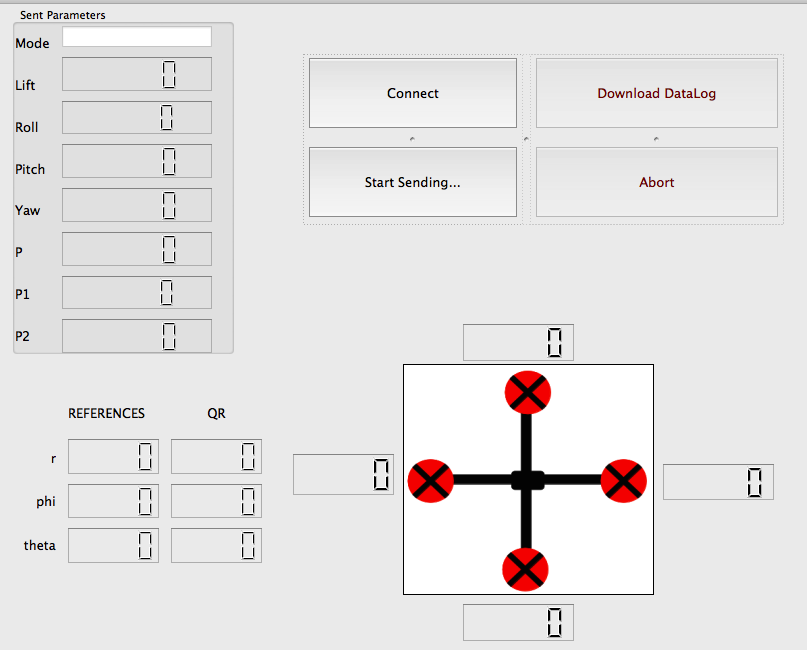
\includegraphics[scale=0.4]{Figures/GUI.png}
	\caption{Designed User Interface}
	\label{fig.GUI}
\end{figure}

\begin{table}[ht]
\centering
\begin{tabular}{|c|c|}
\hline 
\textbf{Button} & \textbf{Functionality} \\ 
\hline 
\hline 
Connect / Disconnect & Establishes communication with the QR (through RS232). Once established, \\ & the \emph{Start Sending} button is enabled\\ 
\hline 
Start/Stop Sending & Data is sent and received. Joystick/Keyboard commanded inputs and Telemetry \\ & are displayed  where indicated. 
\\ & Connect button (now labeled as Disconnect) is disabled until the \\ & button is pressed again.
\\ & \emph{Abort} and \emph{Download DataLog} are enabled
\\
\hline 
Download DataLog & \texttt{EXIT\_MODE} is sent to the QR and data is received and stored in a \texttt{.txt} file
\\ & \emph{Start/Stop Sending} button is disabled while data is retrieved\\
\hline 
Abort & \texttt{ABORT\_MODE} is sent to the QR setting all engines to zero\\ 
\hline 
\end{tabular} 
\caption{GUI functionalities}
\label{tbl:GUIButts}
\end{table}

Telemetry data is shown in 3 display controls (QR column with r, phi, theta) next to the commanded values \texttt{REFERENCES} which are only displayed in \texttt{FULL\_CONTROL} mode. All commanded signals from the keyboard and joystick are shown in the Lift, Roll, Pitch, Yaw, P, P1, P2 controls as well as the set MODE. The \texttt{P} values are only changed in \texttt{YAW\_CONTROL} and \texttt{FULL\_CONTROL} modes as explained in Section \ref{sec:modeselection}. Four extra indicators show the expected motor speed (Along with a QR schematic for easier understanding). The PC calculates these motor speed values in function clones from the FPGA functions, locally on the PC by using the same input data. As a safety measure, the QR must be set in \texttt{SAFE\_MODE} before communication is stopped (using the \emph{Start/Stop Sending} button). If the user terminates the program, \texttt{SAFE\_MODE} is set in the QR and the RS232 port is closed.

%-------------------------------------------------------------------------------------------------------------------------------------------------------------------------------------

\subsection{Memory allocation in the FPGA}
As opposed to the FIFO buffers in the example code provided for the QR, \textbf{Imara} implemented circular buffers. These buffers are preferred as they only overwrite current values when packets are received faster than they are handled, which is something we can adjust. The FIFO buffer did not recognize a lot of packets as these were broken up when reaching the final element of the buffer, favoring the use of a circular buffer. The buffers are type defined as a \texttt{CBuffer struct} including its \texttt{size}, the oldest element \texttt{start}, its newest element \texttt{end} and a vector of \textsc{byte} elements \texttt{$^*$elems}.

The circular buffers are initialized for the transmitting and receiver buffer as well as for the data log buffer which needs a different size range. To generally allocate memory, the \texttt{calloc()} function would be used after which the buffers can be released. The \textsc{x32} library however does not support these functions and needs a work around. To accommodate for this, global arrays with the preferred circular buffer sizes are initialized upon the start of the system. In stead of initializing the vector of elements of the circular buffer in the \texttt{cbInit()} function, we pass the address of the matching global array and position the vector of elements in the address of the array.  To make sure the circular buffers are empty when entering the main \texttt{while()} loop, the buffers are cleaner using the \texttt{memset()} function in \texttt{cbClean()} as coded by \textbf{Imara}.

The writing macro \texttt{cbWrite} works by writing a value to the newest element of the circular buffer, repositioning the pointer to the current newest element. It then double checks whether the buffer is full and if so overwrites. The checksum is then appended because the address of its variable is passed in the function. Although changing the functionality to a macro decreased the time for saving in the buffer from 91 $\mu$s to 64 $\mu$s and the total amount of time to 1738 $\mu$s to 984 $\mu$s. Sending a single byte previously took 150 $\mu$s to perform, while it only takes 83 $\mu$s using the macro. These timing specifications are further elaborated in Section \ref{sec:conclusion}.

%-------------------------------------------------------------------------------------------------------------------------------------------------------------------------------------
% All info considering communcation protocols
\subsection{Communication Protocols}
As mentioned in Section \ref{sec:architecture}, the different interfaces require different communication protocols to perform optimal communication. This section discusses these protocols. 

%-------------------------------------------------------------------------------------------------------------------------------------------------------------------------------------

\subsubsection{Pc2Fpga}
In order to efficiently transmit  data from the PC to the FPGA, a simple and compact communication protocol was implemented. It consists of a fixed length 7 bytes packet, including a starting byte \textbf{0x80}, 5 parameters and a checksum to ensure a reliable communication (Table \ref{tbl:PkgDefinition}). \todo{add calculation to how many bytes can be send using the baudrate of 115k2bps 8n1}

In order to be able to receive on the RS232 line, the \texttt{INTERRUPT\_PRIMARY\_RX} has to be enabled. This done in the initializing of the interrupts in the main loop. 

\begin{table}[ht]
\centering
\begin{tabular}{|c|c|c|c|c|c|c|}
\hline 
0x80 & MODE & LIFT/- & ROLL/P & PITCH/P1 & YAW/P2 & CHECKSUM \\ 
\hline 
\end{tabular} 
\caption{Packet Definition in bytes}
\label{tbl:PkgDefinition}
\end{table}

Although data from the joystick comes in the [$2^{15}$,$2^{15}-1$] range, a single byte is used for each parameter. This is enough taking into account that high sensitivity from the joystick is not needed and rather undesirable (may introduce noise).

The packet structure is composed of
\begin{itemize}

\item{\emph{Starting Byte} \textbf{0x80}, none of the parameters nor the checksum are allowed to have this value.}

\item{\emph{Mode} is set in the second byte as an unsigned char.}

\item{\emph{Lift} is scaled from $[0-255]$ excluding 128 (\textbf{0x80}).}

\item{\emph{Roll}, \emph{pitch} and \emph{yaw} are scaled in the range $[-127,127]$, and then type-cast to unsigned char. The same range is used to scale the control gains (\emph{P} (for yaw control), \emph{P1} and \emph{P2} (for full control)).}

\item{\emph{Checksum} is calculated as a two's complement addition of all parameters (exluding the starting byte). The \textbf{0x80} value is handled and changed to \textbf{0x00}.}

\end{itemize}

The parameters encapsulated in the packet depend on the selected mode. \emph{Panic, Manual, Calibration,Yaw Control} and \emph{Full Control} modes include \emph{lift}, \emph{roll}, \emph{pitch} and \emph{yaw} as parameters. The \emph{P} mode includes an empty byte $'0'$, \emph{P} (for yaw control) and \emph{P1} and \emph{P2} (for full control) gains as parameters (Table \ref{tbl:PkgDefinition}). Although \emph{lift}, \emph{roll},\emph{pitch} and \emph{yaw} are transmitted for safe, panic and calibration modes, they are not acknowledged by the FPGA as discussed in the next section \todo{still refer to main code of fpga loop}. Data coming from the joystick and keyboard are scaled in $[0-255]$ range and encapsulated in a single byte (\emph{unsigned char}) per parameter.

A data structure is implemented in the \emph{Package.h} file. This structure includes functions to initialize, set parameters into the packet and calculate the checksum. Some extra functions are included to clip the data to the [-127,127] range and handle \textbf{0x80} exceptions. This simple communication protocol structure allows for more efficiently decoding in the FPGA, handling always the same packet length.

%-------------------------------------------------------------------------------------------------------------------------------------------------------------------------------------

\subsubsection{Mode selection}
\label{sec:modeselection}
To assess the mode changes requested by the user, the \texttt{mode\_selection()} function is executed between readings of the keyboard and the communication packet creation. The QR operation is always started in \textit{safe mode} and any change between modes must first pass by this safe state. Exception is made to access \textit{panic mode} or \textit{abort mode} as a safety measure. In order to change from \textit{safe mode} to an intended control mode there are two main checks: \textit{Lift} and the sum of the engine values must be equal to $0$, which is equivalent to have all the 4 engines set to $0$. The latter check is done by reading the third least significant bit of the fpga status(\textbf{TELEMETRY FLAG}), received in the telemetry packet, a byte appended in the telemetry send by the QR. 

Moving to both \textit{yaw-controlled mode} and \textit{full control mode} requests an extra check to assess if the sensors calibration was already performed. This \texttt{Calibration\_Done} flag is represented in the least significant bit of the byte. Changing between a control mode and the \textit{P control mode} is enabled to adjust the proportional gains (\textit{P,P1,P2}) of the controllers. Mode changes to \textit{safe mode} are performed automatically when \textit{panic mode} or \textit{calibration mode} have completed its functionality. This \texttt{Safe\_Mode\_Request} is also appended in the telemetry flag. 

Any time an attempt is made to change mode and all the requirements are not fulfilled, the communication packet sends the previous operating mode which is saved in the variable \texttt{prev\_mode} locally on the PC.

Including the mode selection in the PC side allows to avoid all the needed checks in the FPGA. The cost of including one extra byte (\textbf{TELEMETRY FLAG}) in the telemetry packet revealed to be a rather advantageous solution in terms of processing time in the FPGA. \worries{do we have to specify this, I think so}

\begin{table}[h]
\centering
\begin{tabular}{|c|c|c|c|c|c|c|c|}
\hline 
DC & DC & DC & DC & DC & ENGINES NULL & SAFE MODE REQUEST & CALIBRATION DONE \\
\hline 
\end{tabular} 
\caption{TELEMETRY FLAG Definition in Bits}
\label{tbl:TelFlagDef}
\end{table}

%-------------------------------------------------------------------------------------------------------------------------------------------------------------------------------------

\subsubsection{Fpga2Pc}
To supervise the behavior of the QR, telemetry is send on the same RS232 line. To ensure a reliable a starting byte and checksum as discussed in the next section is appended in the packet. The telemetry sends the most important features to supervise: the angular rate $r$ for yaw-control and the angular velocities $\phi$ and $\theta$ to distinguish the motion of the QR.  \todo{need to detail why just these}. Phi and theta \todo{are both this many bytes and therefor we need 2 bytes to be send etc} Along with these parameters, the status of the FPGA, appended in the \texttt{TELEMETRY\_FLAG} is sent as defined in Table. \ref{tbl:TelPkgDefinition} 

As the final telemetry coded by \textbf{Imara} takes 904 $\mu$s to assign and send, it will claim the RS232 line, slowing down the entire process. For this reason a polling technique was implemented. The \texttt{send\_telemetry()} is called in every while loop, but checks whether or not the defined \texttt{POLLTIMEMS} of 200 $ms$ is passed. If this is the case, the telemetry flag is set according to the sum of the engines. The appropriate parameters are then written to the transmitting circular buffer using the macro function \texttt{cbWrite()} as written by \textbf{imara} which immediately updates the checksum by passing the address of the local variable. If the checksum contains the starting byte \textbf{0x80}, it is appended to \textbf{0x00}. The checksum is then added to the packet after which a while loop iterates until the transmitting buffer is empty (\texttt{txcb.end == txcb.start}). Until then it waits indefinitely for the RS232 to change its status register to \texttt{X32\_rs232\_stat \& 0x01}, indicating it is ready to send the next byte upon which it does so by using the macro \texttt{cbGet()} as written by \textbf{Imara} which writes the current value of the transmitter buffer to the address of the \texttt{X32\_rs232\_data} RS232 data register, initializing the transmission of the written byte. 

\begin{table}[ht]
\centering
\begin{tabular}{|c|c|c|c|c|c|c|c|}
\hline 
0x80 & r & phi $>>$ 8 & phi & theta $>>$ 8 & theta & TELEMETRY FLAG & CHECKSUM \\
\hline 
\end{tabular} 
\caption{Telemetry Packet Definition in Bytes}
\label{tbl:TelPkgDefinition}
\end{table}

In order to be able to send on the RS232 line, the \texttt{INTERRUPT\_PRIMARY\_TX} has to be enabled. This done in the initializing of the interrupts in the main loop. 

Initially the \texttt{send\_telemetry()} was coded by \textbf{Imara} to send only the first byte of the telemetry, causing the initiation of the \texttt{isr\_rs232\_tx()}. The next byte to be send in the circular buffer would this way be put in line waiting to be handled by a scheduler, causing no delays for other important ISRs. This would initiate a new interrupt for every byte send until the buffer was empty. Due to a shortage of team members and time we decided to send all telemetry in one go instead

\todo{check whether or not it makes a difference when sending local or global variables}

%-------------------------------------------------------------------------------------------------------------------------------------------------------------------------------------
% Reliable communication
% 

\subsection{Communication properties}
\subsubsection{Reliability} 
To ensure a \emph{reliable communication}, the sent packets are appended with a checksum.  This checksum is calculated at both the PC and the QR. When the locally calculated checksum does not match the send checksum, the package is regarded as faulty and discarded. The checksum in the \textsc{Pc2Fpga} protocol is calculated using a \emph{two's complement addition checksum} as it has been used before in a previous project by \textbf{Daniel}. The checksum calculation used in the telemetry and data logging written by \textbf{Imara} uses the \textsc{XOR} checksum.  

The two's complement method takes 22 $\mu$s for every addition and requires a complement taking 5 additional $\mu$s while the \textsc{XOR} method takes 22 $\mu$s for every \textsc{XOR}'ing. The \textsc{XOR} checksum has a \emph{Hamming Distance} of 2, detecting all one-bit errors, but not all two-bit errors. This happens when an even number of bit errors occurs in the same bit position of the checksum computational block. The two's complement addition with a Hamming Distance of 2 can be seen as an improvement of the \textsc{XOR} checksum as it mixes between bit positions of the data-blocks as a result of the bit-by-bit carry outs of the additions. As most of the control loop delay is caused by the X32 code, we want to limit the amount of instructions. Because of this and it's data independence we decided to use the \textsc{XOR} checksum 

\subsubsection{Dependability}
Whenever the PC link is broken or disconnected, the code should immediately signal the error and enter panic mode. \textbf{Imara} coded this using a communication counter \texttt{commflag} which is set to zero whenever a package is received in the interrupt service routine of the RS232 RX of the FPGA. Whenever the counter exceeds the threshold \texttt{commthres}, the mode is set to \texttt{PANIC\_MODE}. 

\subsubsection{Robustness}
\todo{write arithmetic solutions for representing and handling of sensor values}

%-------------------------------------------------------------------------------------------------------------------------------------------------------------------------------------
% Safety mode, emergency stop, stalling proof, robust to noise, reliable communication, 
% dependability, robustness

\subsection{Safety features}
The \emph{safe mode} is the initial mode in which the QR operates and has to be accessed in between switching modes. \textbf{Imara} coded the safe mode function in the matching header file in which the FPGA's status is updated in the \texttt{telemetry\_flag} as discussed in Section \ref{sec:safemode}. This safe mode and the \texttt{mode\_selection()} function ensures that no illegal control values are send to the engines when switching modes. 

An extra \texttt{abort\_mode} was created by \textbf{Diogo} to distinguish between directly dangerous situations where the FPGA should shut down the engines and shut down and situations where the system can reduce engine values in a controlled manner such as the \texttt{panic\_mode} provides. \todo{Diogo, can you support the reasons for this}

To prevent stalling to occur in the brushless engines, a \texttt{check\_motor\_ramp()} function is called in the PC after the \texttt{mode\_selection()} performs the mode selection. This function written by \textbf{Daniel} clips the ramping up of the engines to a set maximum value for increasing and decreasing of the engine values. This is done by comparing current \texttt{lift} control values with a \texttt{prev\_lift}. 

%-------------------------------------------------------------------------------------------------------------------------------------------------------------------------------------
%   Datalogging
\subsection{Data Logging}

Data logging as coded by \textbf{Imara} is used to verify the filtering/controller behaviour, as well as QR behaviour in general. The \textsc{store\_data()} function polls in the same way as the \texttt{send\_telemetry()} function does, but instead every \textsc{DATASTORETIMEMS} of 150 $ms$. The 33 bytes packet is composed of a starting byte (\textbf{0x80}), 16 parameters (31 bytes) and a checksum. Logged data includes a timestamp (1 byte), MODE, Lift, Roll, Pitch and Yaw (1 byte each), motor commanded speeds (2 bytes each), sensor normalized data (1 byte each) excluding acceleration reading in Z direction, phi and theta angles (2 bytes each), p and q angles (1 byte each), P, P1 and P2 control gains (1 Byte each) and control time (1 byte). The packet is composed in the \textsc{store\_data()} function. \todo{specify why we need these and not others}

In contrary to the telemetry, the data log is send on command when the \emph{exit mode} is triggered (Pressing Del key or clicking in the Data Log button in the GUI). The FPGA exits the while loop and starts sending the stored data in the \textsc{send\_data()} function which keeps sending until the circular data log buffer is empty. In the mean time the PC stops writing in the port and starts receiving from the fpga. As the data is received, the PC checks for the start byte (\textbf{0x80}) and stores the subsequent bytes until the expected size is reached (33 bytes). Once the complete packet is stored, the checksum is verified and the packet is written into a text file. All packets are separated by a CR and the starting byte is excluded (as the packet is verified before is written into the file).

A matlab script is used to decode and visualize the logged signals.\todo{daniel, write about the matlab code}


%-------------------------------------------------------------------------------------------------------------------------------------------------------------------------------------
%   Filtering
\subsection{Filtering}
\label{sec:filtering}

QR sensor signals must be filtered and bias-cleared before they are feed in the controller. Figure \ref{fig.Noise} shows signals in steady state coming from the accelerometer and gyroscope. Two filter options are explored to perform the signal reconditioning: Butterworth Filter and Kalman Filter developed by \textbf{Daniel} and \textbf{Diogo}, respectively.

The only control mode that makes use of the sensor filtered values is the \textit{full control mode}, since the \textit{yaw rate} \texttt{r} for the \textit{yaw control mode} can be read directly from the gyro sensor along the respective axis. Hence, it was decided to include the sensor reading and filtering in the main \texttt{switch case} along with the \texttt{case FULL\_CONTROL\_MODE}. Other options were considered such as including the sensor handling in a timer interrupt or in the \texttt{isr\_qr\_link} interrupt. However, for both cases sensor reading and filtering would be performed even in unnecessary conditions. Moreover, setting it just before the \texttt{full\_control\_mode()} function allowed to keep the sensor handling at an approximately constant frequency, what is of importance for a good performance of the filters. In the case of changing to a different mode, the filter's constants are reinitialized so that erroneous values are not obtained if \textit{full control mode} is executed after.

\begin{figure}[ht]
\centering
%	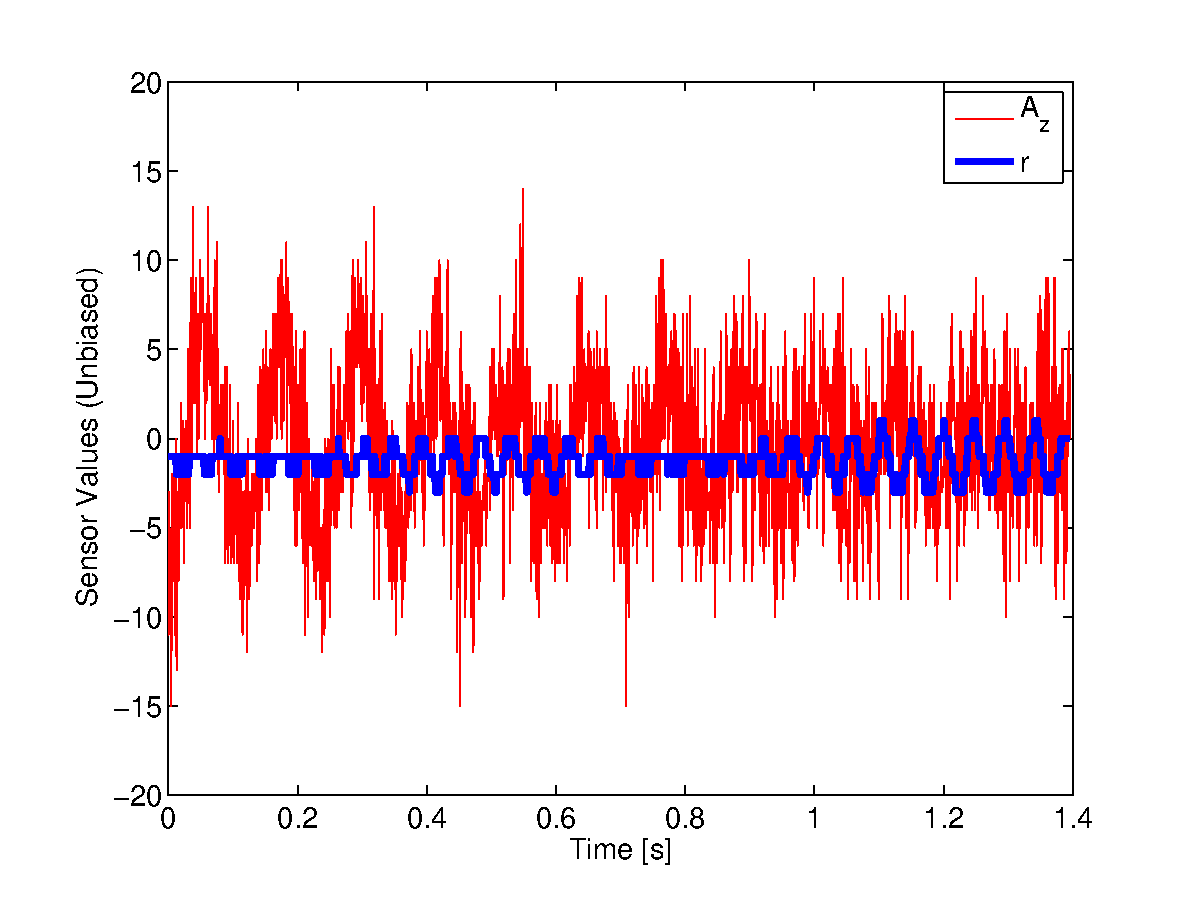
\includegraphics[scale=0.6]{Figures/Noise.eps}
	\caption{Accelerometer vs Gyro signals noise comparison}
	\label{fig.Noise}
\end{figure}

\subsubsection{Butterworth Filter}

A first order Butterworth filter is used to perform noise reduction. This noise reduction can be regulated setting the cutoff frequency. Lower cutoff frequencies will lead to a much smoother signal with delay as trade-off. In contrast, higher cutoff frequencies results in a synchronized signal with still some noise (Figure \ref{fig.NoiseComp}). Although a lower cut frequency (10Hz) lead to a delayed signal, the phase shift for a Butterworth $1^{st}$ order is less than $90^{o}$ at the cut frequency, making it suitable for the QR application. 

\begin{figure}[ht]
\centering
%	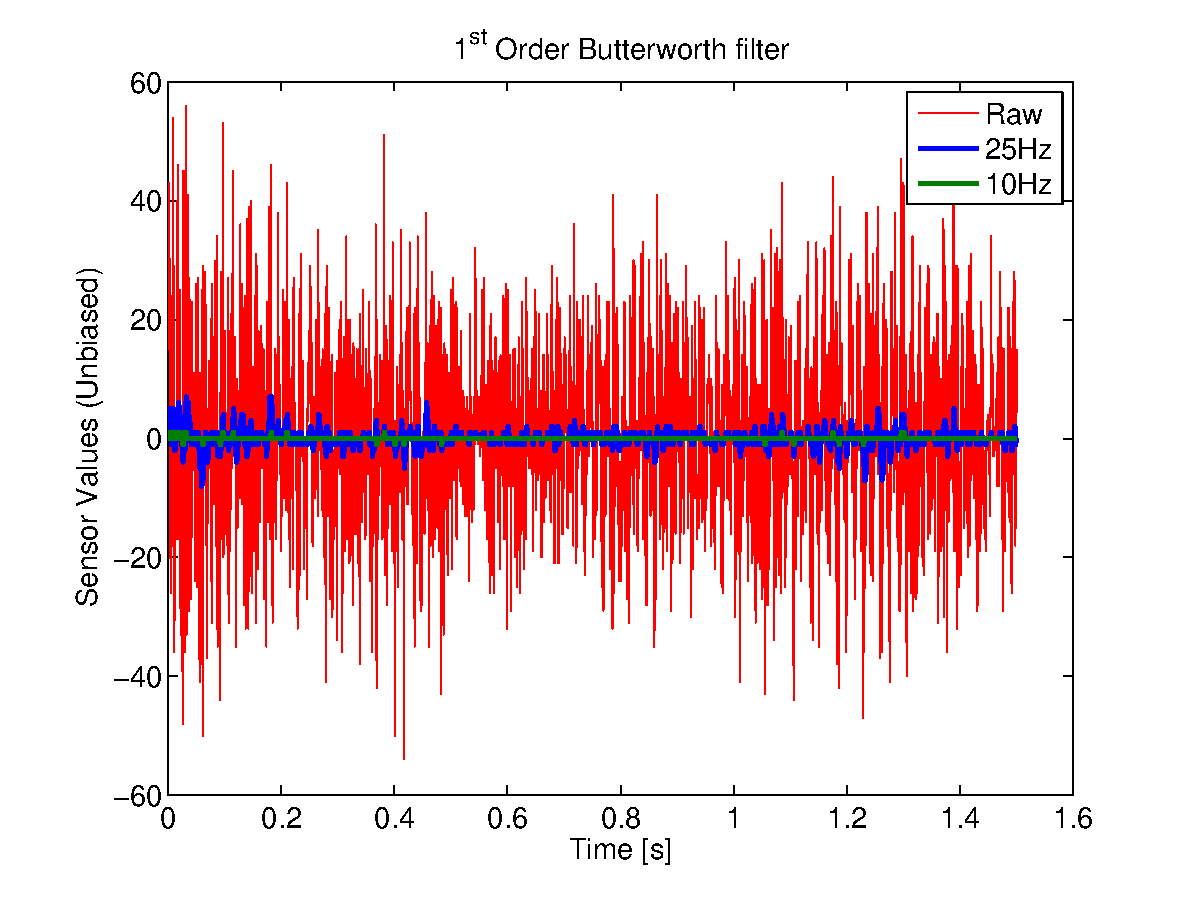
\includegraphics[scale=0.6]{Figures/NoiseComp.eps}
	\caption{Cutoff Frequency effect in a $1^{st}$ order Butterworth filter}
	\label{fig.NoiseComp}
\end{figure}

Implementation of a $1^{st}$ order Butterworth filter is straightforward compared to a Kalman filter. Given the signal sample frequency and the desired cutoff frequency, a set of constants ($A_0$, $A_1$, $B_0$ and $B_1$) are calculated. Using this constants the filtered signal is reconstructed out from the raw sensor values (current and previous) and the previous filtered value.

\begin{equation}
	 B_0 y_k = A_0 x_k + A_1 x_{k-1} + B_1 y_{k-1}
	 \label{eq:Butt1st}
\end{equation}

Equation \ref{eq:Butt1st} shows the update formula for a 1st order Butterworth filter, where $x$ and $y$ are the raw and filtered values respectively, $A_0$, $A_1$, $B_0$ and $B_1$ are the constants for a $1^{st}$ order Butterworth filter, $k$ and $k-1$ represent the current and previous measurement.

The calculated constants for the $1^{st}$ order Butterworth are rational numbers and a proper scaling is applied in order to compute the multiplication with the measured and filtered values (The FPGA soft core does not handle floating point numbers). A 14 bit fix point arithmetic is applied in this case to compute the constants (This is multiply by $2^{14}$ and round the number as seen in Table \ref{tbl:ButtConstants}). \todo{this has to be explained more thoroughly, the arithmetics}

\begin{table}[ht]
\centering
\caption{Telemetry Packet Definition}
\begin{tabular}{|c|c|c|c|c|}
\hline 
 & $A_0$ & $A_1$ & $B_0$ & $B_1$ \\ 
\hline 
Real Values & 0.0242 & 0.0242 & 1 & -0.9515 \\ 
\hline 
14 Bit Fix Point & 396 & 396 & 16384 & -15590 \\ 
\hline 
\end{tabular}
\label{tbl:ButtConstants}
\end{table}

Once the values are scaled properly multiplication can be computed as the product of two integers dividing the result by $2^{14}$ (This is made using the $>>$ operator). The outcome of the multiplication is used to compute the filter described in equation \ref{eq:Butt1st}. To generate a speed up of the Butterworth function, a marco was coded by \textbf{Imara} for the \texttt{mult(a, b)} function. 

\subsubsection{Kalman Filter}

The Kalman filter is applied for correction of the sensor reading errors related to gyroscopes drift and accelerometers noise. An extra effort for noise reduction is done by using the Butterworth filter, as stated in the previous section. \todo{have to declare that this causes a delay of 180 degrees and was actually an error in our code}

The algorithm applied was the same as presented in the course lectures. A first approximation of the angle and associated rate is found by directly reading the accelerometer and gyroscope values, respectively. A estimate of the angle is attained by integrating the angle rate using the constant \texttt{P2PHI}. Then, an iterative correction of that value is performed by using constant \texttt{C1} and comparing the actual estimate and accelerometer reading. Also the value obtained for the angle rate is corrected in a similar way by the constant \texttt{C2}, which will influence the rate integration in the following iteration. By adjusting the values of the referred constants, we define the weight or influence that each sensor reading has in the angle and rate computation. This continuous iterative process will correct for both accelerometer noise and gyroscope drift in the long term.

In order to achieve a faster algorithm the constants \texttt{C1} and \texttt{C2} are defined as a power of $2$ value such that the introduced corrections can be performed by a simple shift right. In the integration step of the algorithm the constant \texttt{P2PHI} was first implemented by using an estimate value and applying the fixed point arithmetic, defined in the previous section. Later, for easing the tuning process it was also tried to implement the integration by applying shift rights to the angle rate instead of using the multiplication by \texttt{P2PHI}. The tuning procedure of the Kalman Filters was not completed, therefore final values of the constants were not found as will be explained in section \ref{sec:results}.


%-------------------------------------------------------------------------------------------------------------------------------------------------------------------------------------
%   Control Modes
\subsection{Control Modes(\todo{Diogo Monteiro})}

\subsubsection{Safe Mode}
\label{sec:safemode}
The \textit{Safe mode} as developed by \textbf{Imara} is responsible for de-energizing the four rotor engines. The engine values are decreased using a \texttt{SAFE\_JUMP} value of 5 to avoid stalling of the engines whenever the FPGA operates in safe mode as determined in the \texttt{switch case} in the \texttt{main} function. The mode can be accessed by pressing '$0$' in the keyboard and had to be accessed before any mode change with the exception of \texttt{Panic\_mode} and \texttt{Abort\_mode}.

\subsubsection{Panic Mode}
\textit{Panic mode} developed by \textbf{Diogo} can be accessed by pressing '$1$' in the keyboard. The main purpose of this function is to allow the safe landing of the QR in a lost of control scenario. To achieve this, a mean of the actual engines values is computed and in case it is higher than an experimentally defined \texttt{LIFT\_THRESHOLD}, a progressive balance of the four engines is accomplished through changes by a value of $30$ (\texttt{ENGINE\_STEP}) until the reference threshold is attained for each engine. The value \texttt{LIFT\_THRESHOLD} was found by increasing lift until the QR was about to hover.  In case the mean value of engines is superior to the \texttt{LIFT\_THERSHOLD}, the final reference becomes the computed mean. This was done to avoid sudden increases of engines thrust whenever panic state is reported. The value chosen for the \texttt{ENGINE\_STEP} revealed to be fairly adjusted to the requested engine speed changes and at the same time stalling proof.

Finally, when all the engines are at the same speed a delay time of 2 seconds is performed in order to allow the balancing of the QR. After, the \texttt{TELEMETRY\_FLAG} is updated to request a change to \textit{safe mode}.

\subsubsection{Manual Mode}
\textit{Manual mode} developed by \textbf{Diogo} can be accessed by pressing '$2$' in the keyboard. In this mode a direct mapping between the received information and the engine values was designed. A initial base value to the engines is assigned using the \textit{Lift} information, by defining a scaling between $[0-255]$ and $[0-\text{\texttt{ENGINE\_LIMIT}}]$. In order to obtain a faster increase of the engines until an approximate hover state is attained, two different linear scaling were defined: one for \textit{Lift} values up to $75$ (\texttt{LOW\_LIFT\_CONVERSION}) and second for the rest of the range (\texttt{HIGH\_LIFT\_CONVERSION}).

The other received parameters (\textit{Roll, Pitch, Yaw}) will then apply offsets to the base value defined, such that the intended movement by the user can be performed. For the case of \textit{Roll} and \textit{Pitch}, only one engine is affected for each information. This allows to approximately maintain a constant lift force in the QR. For the \textit{Yaw} case and due to the same reason, all engines suffer symmetric offsets. The scaling of the latter parameters is done between $[-127,127]$ and $[-50,50]$, which is defined in the code using the macro \texttt{ROLLPITCHYAW\_ENGINE\_LIMIT}. 

Note for the fact that when the reference value is negative($[-127,0[$), a signing typecast is performed since the decoded information in the fpga is unsigned. This typecast is also performed for the controlled modes.

\subsubsection{Calibration Mode}
\textit{Calibration mode} developed by \textbf{Diogo} can be accessed by pressing '$3$' in the keyboard. In order to compute the calibration values of each sensor, the function \texttt{calibration\_mode()} is called continuously until 256 (\texttt{CALIBRATION\_THRESHOLD}) values of each sensor reading are saved and summed in the array variable \texttt{OFFSET\_x0[i]} with 6 positions (6 sensors). When the sum is finished, what is controlled by the counter \texttt{calibration\_counter}, a shift right of $8$ ($2^8=256$) bits is performed to obtain the final offset calibration values. At this point the \texttt{TELEMETRY\_FLAG} is also updated to request a change to safe mode in the PC and inform that calibration was already performed.

\subsubsection{Yaw-Controlled Mode}
\textit{Yaw-Controlled Mode} developed by \textbf{Diogo} can be accessed by pressing '$4$' in the keyboard. For the development of this mode, a linear approximation of the QR dynamics was used in order to avoid the necessity of creating a square-root routine needed for the fidelity model of the system, presented in the assignment description. Despite the approximation, the controller behaviour proved to not be deeply affected and still bringing the reference error to null.
For this control mode the lift, roll and pitch movements are still considered manually controlled, therefore a similar scaling to the one used in \texttt{manual\_mode()} was applied. However, instead of a direct scaling of the engines values here it is done for the \textit{lift force} \texttt{Z} ,\textit{roll momentum} \texttt{L} and \textit{pitch momentum} \texttt{M}. All the definitions used for the scaling constants were based on the values used in the manual mode, which were tuned experimentally. This way, the expected behaviour of the QR is closely related to the one applied in the \textit{manual mode}, except for the yaw motion.

For the \textit{yaw momentum} \texttt{N} the proportional control loop is applied based on the sensor reading of the yaw rate \texttt{r}. This is done by a direct reading of the sensor \texttt{x0[5]} corrected by the calibration. Having the force and momentums defined, the inversion of the linearized system dynamics is performed in order to obtain the engine values. 

\subsubsection{Full Control Mode}
\textit{Full Control Mode} developed by \textbf{Diogo} can be accessed by pressing '$5$' in the keyboard. This mode follows the same algorithm used for the \textit{yaw-controlled mode} but with only a direct scaling for the \textit{lift force} \texttt{Z}. Also the definition of the \textit{yaw momentum} \texttt{N} is the same used in the previous controlled mode. 

For both the \textit{roll momentum} \texttt{L} and \textit{pitch momentum} \texttt{M}, a proportional (\texttt{P1}) and derivative (\texttt{P2}) controller is applied based on the actual values of the roll and pitch dynamic angles and rates. This angular states are provided by the sensor reading after passing through the filters, as explained in \ref{sec:filtering}. In the end the linearized system dynamics are inverted and the engines values computed.

\subsubsection{P Control Mode}
\textit{P Control Mode} developed by \textbf{Diogo} can be accessed by pressing '$6$' in the keyboard. This mode is intended to be accessed when an adjustment of the controllers parameters is requested for tuning purposes. Initially the parameters are defined using the macros \texttt{PCONTROL\_INIT}, \texttt{P1CONTROL\_INIT} and \texttt{P2CONTROL\_INIT}. When this mode is entered an offset can be applied to the initial values based on the received in the communication packet. The range of change is set between $[\text{\texttt{\_INITIAL}}-127,\text{\texttt{\_INITIAL}}+127]$.

\subsubsection{Abort/Exit Mode}
\textit{Abort/Exit Mode} developed by \textbf{Diogo} can be accessed by pressing \texttt{DEL} in the keyboard or pressing 'strike' button in the joystick. The option to use \texttt{DEL} key instead of \texttt{ESC} was due to safety measures, as the latter button is close to the mode definition keys. 

The main function of this mode is to permit the exiting of the main loop in the fpga. It also allows a faster shutting down of the engines as an emergency measure, in case \textit{panic/safe} mode are not an option. The exiting is done by incrementing the flag \texttt{program\_done}.




%----------------------------------------------------------------------------------------
%	EXPERIMENTAL RESULTS
%	list the capabilities of your demonstrator
%----------------------------------------------------------------------------------------

\section{Experimental results}
\label{sec:results}
In the demonstration performed in the last laboratory session, we were able to show the capabilities of the QR running the code developed. In this section we discuss what worked correctly and also what went wrong. Some reasoning is as well applied to try to justify what caused those failures and understand what further work should be done in order to correct them.

The first test performed was to the mode change allowance possibilities. Here, it was verified that all the several safety requirements were fulfilled. Nonetheless, one issue was identified when the \textit{calibration mode} was selected and the automatic change back to safe state was not performed. Forcing a change by pressing '$0$' seemed to work and later when \textit{calibration mode} was called again, everything performed as expected. Although further debugging was needed to identify the issue source, it seemed to be related with a wrong initialization of the \texttt{TELEMETRY\_FLAG}.

The execution of the \textit{manual mode} worked perfectly, as the QR revealed an accordingly behaviour with the user references. It also showed a smooth performance in roll, pitch and yaw movements revealing the proficient tuning of the scaling functions.\todo{WE SHOULD TALK ABOUT THE LAG BUT I DONT KNOW HOW WE SHOULD JUSTIFY IT}. At this point we also had the chance to test the \textit{panic mode} and \textit{safe mode}, which executed their tasks as expected taking the QR to a safe and steady state. The following assessment was done to the \textit{calibration mode}. We could notice that the sensors offset was found correctly since the user interface showed null values for the dynamic angles and rates after calibration and when one of the controlled modes was accessed.

At this point we were in condition of testing the \textit{yaw-controlled mode}. A first approach was done by leaving the yaw rate \texttt{r} set to 0 and applying a rotational disturbance to check if the reference was followed and attained. As shown in figure \ref{fig:YawControl}, the expected behaviour was accomplished since the QR rapidly rejected the disturbance and followed the reference.

\begin{figure}[ht]
\centering
%	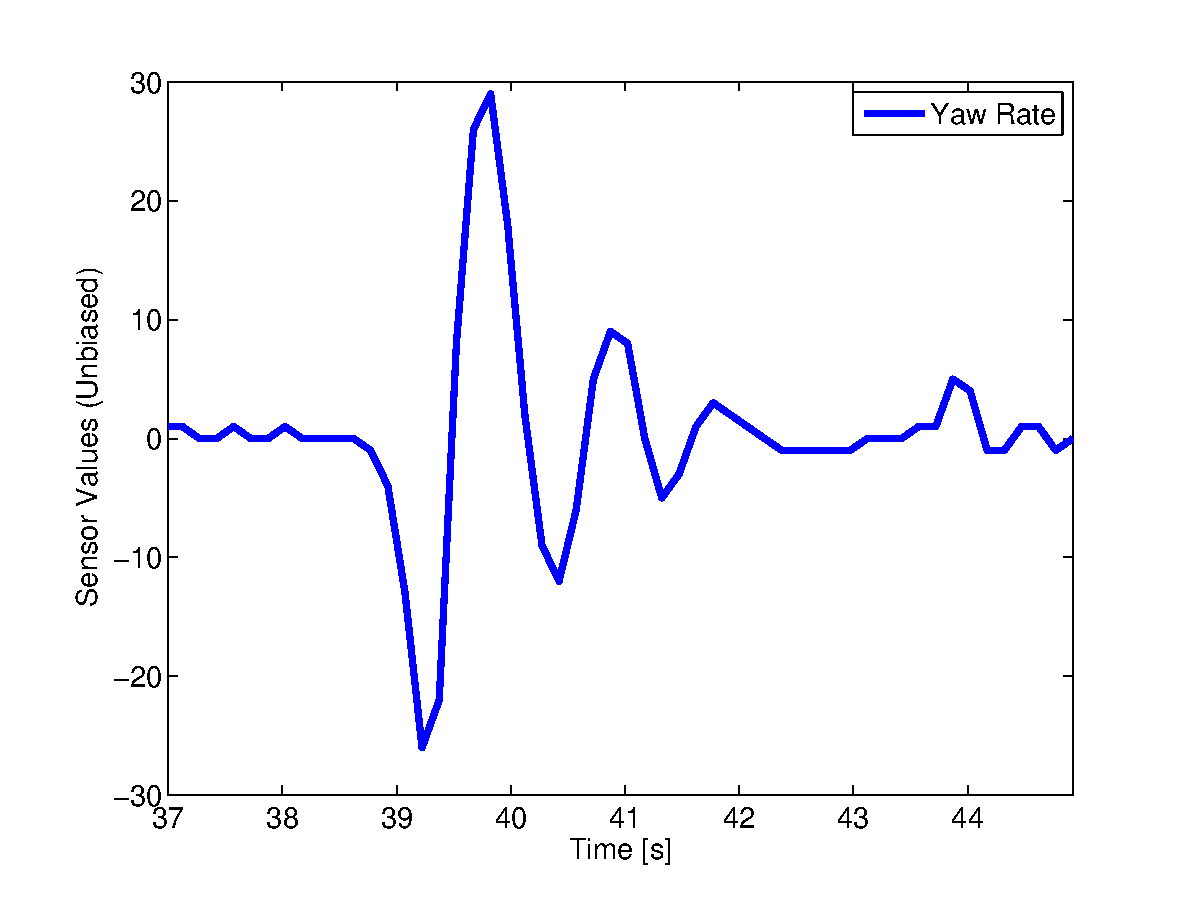
\includegraphics[scale=0.6]{Figures/YawControl.eps}
	\caption{Disturbance rejection in \textit{yaw-controlled mode}}
	\label{fig:YawControl}
\end{figure}

Despite this successfully test, when a different reference (provided by the joystick) was feed to the controller a strange behaviour was witnessed. Basically, the controller was assuming a symmetric reference to the one intended. The error here was identified in the dynamics inversion of the mode algorithm. The linearized dynamics were established using as convention a positive \textit{yaw momentum} \texttt{N} for a clockwise rotation (when looking from above the QR), while the reference yaw rate definition used the opposite definition. This issued could be easily solved by adding a minus sign to the \texttt{N} equation of the linearized system.

Since the group did not have the chance to properly tune the Filtering parameters it was decided not to test \textit{full control mode} since an unexpected and not safety behavior could be experienced. Nevertheless, assuming that the algorithm used clearly resembles the applied for the \textit{yaw-controlled mode}, we believe that it was correctly implemented.

\todo{Talk about GUI\\}
\todo{Explain why when the cable was disconnected the QR didn't enter panic} 



%----------------------------------------------------------------------------------------
%	CONCLUSION
%	Evaluate the design, team results, individual performance and learning experience
%----------------------------------------------------------------------------------------

\section{Conclusion}
\label{sec:conclusion}


%----------------------------------------------------------------------------------------
%	APPENDIX
%----------------------------------------------------------------------------------------

\newpage
\section{Appendices}

\appendix
\section{Title of Appendix A}
\section{Title of Appendix B}



%----------------------------------------------------------------------------------------

\bibliographystyle{plain}
\bibliography{report}

\end{document}
